\documentclass{amsart}
\usepackage[dvipsnames]{xcolor}
\usepackage{tikz}
\newcommand*{\bigdots}{{\Large $\vdots$}}
\begin{document}
This is a simple document to test out the insertion of annotations on a control PDF.

I'll write a famous test sentence for previewing fonts since it contains every letter in the alphabet.\footnote{There's a term for this: it's \textit{pangram}.}

I should test how different font font sizes interact with the annotations and throw in a figure caption, too.




{\larger[5] The quick brown fox jumps over the lazy dog.}

{\larger[4] The quick brown fox jumps over the lazy dog.}

{\larger[3] The quick brown fox jumps over the lazy dog.}

{\larger[2] The quick brown fox jumps over the lazy dog.}

{\larger[1] The quick brown fox jumps over the lazy dog.}

{\smaller[0] The quick brown fox jumps over the lazy dog.}

{\smaller[1] The quick brown fox jumps over the lazy dog.}

{\smaller[2] The quick brown fox jumps over the lazy dog.}

{\smaller[3] The quick brown fox jumps over the lazy dog.}

{\smaller[4] The quick brown fox jumps over the lazy dog.}

{\smaller[5] The quick brown fox jumps over the lazy dog.}

That is a little unsatisfying that the largest {\tt \string\larger} doesn't fit. Oh well.

\begin{figure}
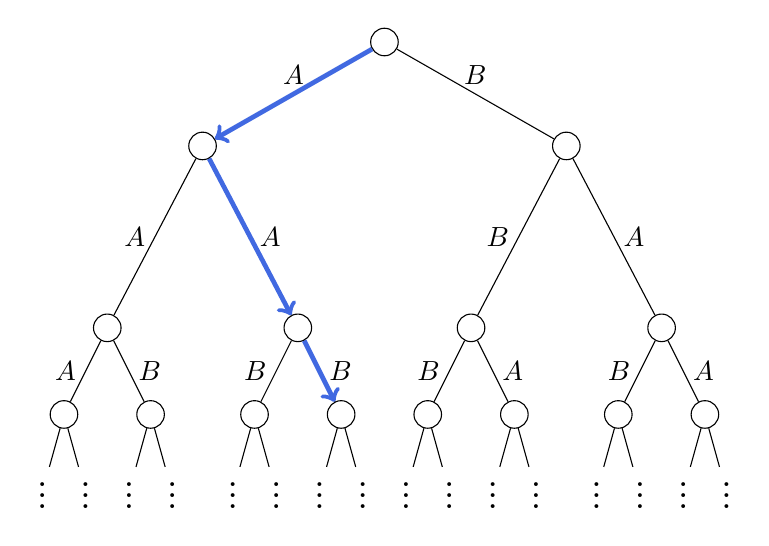
\begin{tikzpicture}
[
    scale = 1.1,
    level 1/.style={sibling distance=42mm, level distance = 1.2cm},
    level 2/.style={sibling distance=22mm, level distance = 2.1cm},
    level 3/.style={sibling distance = 10mm, level distance = 1cm},
    level 4/.style={sibling distance = 5mm, level distance = .9cm},
    ellip/.style={text height = 4mm},
    game/.style={circle, draw, minimum size = .35cm, fill = none},
    whole/.style={draw=black, very thick, inner sep = 25pt, text height = 0mm},
    sub/.style={dashed, draw=black, very thick, inner sep=15pt}, % Style for grouping
    ssub/.style={draw = black, very thick, inner sep = 3pt},
    arrow/.style={draw, ->, color = RoyalBlue, line width = 1.7pt},
]

% Draw the binary tree with an edge label
\node[game] (root) {}
	child {node[game](11) {}
		child {node[game] {}
			child {node[game] {}
				child {node[ellip] {\bigdots}}
				child {node[ellip] {\bigdots}}
			edge from parent node [left] {$A$}
				}
			child {node[game] {}
				child {node[ellip] {\bigdots}}
				child {node[ellip] {\bigdots}}
			edge from parent node [right] {$B$}
				}
	edge from parent node [left] {$A$}
			}
		child {node[game](22) {}
			child {node[game] {}
				child {node[ellip] {\bigdots}}
				child {node[ellip] {\bigdots}}
			edge from parent node [left] {$B$}
				}
			child {node[game](34) {}
				child {node[ellip] {\bigdots}}
				child {node[ellip] {\bigdots}}
			edge from parent node [right] {$B$}
				}
		edge from parent node [right] {$A$}
			}
	edge from parent node [above] {$A$}
	}
	child {node[game] {}
		child {node[game] {}
			child {node[game] {}
				child {node[ellip] {\bigdots}}
				child {node[ellip] {\bigdots}}
			edge from parent node [left] {$B$}
				}
			child {node[game] {}
				child {node[ellip] {\bigdots}}
				child {node[ellip] {\bigdots}}
			edge from parent node [right] {$A$}
				}
		edge from parent node [left] {$B$}
			}
		child {node[game] {}
			child {node[game] {}
				child {node[ellip] {\bigdots}}
				child {node[ellip] {\bigdots}}
			edge from parent node [left] {$B$}
				}
			child {node[game](s) {}
				child {node[ellip] {\bigdots}}
				child {node[ellip] {\bigdots}}
			edge from parent node [right] {$A$}
				}
		edge from parent node [right] {$A$}
			}
	edge from parent node [above] {$B$}
	};
	\draw[arrow] (root) -- (11);
	\draw[arrow] (11) -- (22);
	\draw[arrow] (22) -- (34);
\end{tikzpicture}
\caption{I guess I couldn't help myself from throwing in something complicated looking. But this works out relatively well, actually. Well I don't know. I'm rambinlg to fill up characters on a page.}
\end{figure}

\end{document}
